% ===========================================================================
% Example paper shipped with the physics research template.
%
% Paragraph-level outline (first sentences, in order; together they should
% tell the whole story without the body). Kept visible per the workflow;
% remove only at a hypothetical final submission, do not delete while drafting.
%
%   Abstract  : This is a worked example for the template, not a research
%               result.
%   Intro 1   : The two-body problem under an inverse-square central force is
%               the canonical solvable system of classical mechanics.
%   Intro 2   : The three results below are textbook; the purpose is to
%               demonstrate the template's path from formalism to verified
%               code to a paper.
%   Formalism : A test mass in the field of a fixed central body obeys an
%               inverse-square equation of motion.
%   Integrator: The trajectory is advanced with the velocity-Verlet scheme.
%   Verify    : Four checks, each with a pre-declared falsifier, run as Rust
%               tests.
%   Closing   : This example establishes no new fact about the world.
% ===========================================================================

\documentclass[11pt]{article}

\usepackage[margin=1in]{geometry}
\usepackage{amsmath}
\usepackage{amssymb}
\usepackage{booktabs}
\usepackage{tikz}
\usepackage[numbers]{natbib}
\usepackage[hidelinks]{hyperref}

\title{A worked example: Newtonian two-body orbits with a verified integrator}
\author{First Last\thanks{Replace with the author. This is the example paper
shipped with the template; edit it for your own work or delete it.}}
\date{\today}

\begin{document}
\maketitle

\begin{abstract}
This is a worked example for the template, not a research result. It recovers
three established facts about the Newtonian two-body problem -- the
inverse-square force law, closure of a circular orbit at the Kepler period,
and conservation of the specific orbital energy -- using a small Rust
integrator whose checks run as automated tests. The aim is methodological: to
show how a quantity moves from a stated formalism (stage~3) to code whose
output has been seen against a pre-declared falsifier (stage~4) to a paper in
this template. No new physical fact is claimed.
\end{abstract}

\section{Introduction}

The two-body problem under an inverse-square central force is the canonical
solvable system of classical mechanics, and its closed-form properties make it
a convenient target for checking a numerical method. Reducing the general
two-body problem to a test mass moving in the field of a fixed central body
isolates the central-force dynamics while keeping the algebra short.

The three results reported below are textbook; the purpose here is to
demonstrate the template's path from a stated formalism to code whose output
has been seen against a pre-declared falsifier, and then to this document. The
force law and the gravitational constant are taken from
Newton~\citep{Newton1687} and the CODATA~2018 adjustment~\citep{CODATA2018};
the integrator is the velocity-Verlet scheme~\citep{Swope1982}.

\section{Formalism}
\label{sec:formalism}

A test mass at position $\mathbf{r}$ in the field of a fixed central body at
the origin obeys
\begin{equation}
  \ddot{\mathbf{r}} = -\,\frac{\mu\,\mathbf{r}}{\lvert \mathbf{r} \rvert^{3}},
  \qquad \mu \equiv G M,
  \label{eqn:eom}
\end{equation}
where $G$ is Newton's gravitational constant and $M$ is the central mass. The
magnitude of the force between two point masses $m_1$ and $m_2$ separated by a
distance $r$ is
\begin{equation}
  F = \frac{G\,m_1 m_2}{r^{2}}.
  \label{eqn:force}
\end{equation}
For a bound orbit of semi-major axis $a$, the speed at radius $r$ follows the
vis-viva relation
\begin{equation}
  v^{2} = \mu\!\left(\frac{2}{r} - \frac{1}{a}\right),
  \label{eqn:visviva}
\end{equation}
and a circular orbit of radius $r$ has period $T = 2\pi\sqrt{r^{3}/\mu}$,
which is Kepler's third law.

\section{Numerical integrator}
\label{sec:integrator}

The trajectory is advanced with the velocity-Verlet scheme~\citep{Swope1982}.
For a step $\Delta t$,
\begin{align}
  \mathbf{r}_{n+1} &= \mathbf{r}_{n} + \mathbf{v}_{n}\,\Delta t
    + \tfrac{1}{2}\,\mathbf{a}_{n}\,\Delta t^{2}, \label{eqn:vvpos}\\
  \mathbf{v}_{n+1} &= \mathbf{v}_{n}
    + \tfrac{1}{2}\,\bigl(\mathbf{a}_{n} + \mathbf{a}_{n+1}\bigr)\,\Delta t,
    \label{eqn:vvvel}
\end{align}
with the acceleration
$\mathbf{a}_{n} = -\mu\,\mathbf{r}_{n}/\lvert\mathbf{r}_{n}\rvert^{3}$ from
Eq.~\eqref{eqn:eom}. The scheme is symplectic, so its energy error stays
bounded over many periods rather than drifting secularly; that property is
what the energy check in Section~\ref{sec:verification} measures.

\section{Verification}
\label{sec:verification}

Four checks run as Rust tests in the \texttt{gravity} crate. Each states a
falsifier in advance; the run reports the measured quantity, shown in
Table~\ref{tab:checks} against its bound. The checks use normalized units
($\mu = 1$), except the force-law value, which uses SI units.

\begin{table}[h]
  \centering
  \begin{tabular}{@{}lll@{}}
    \toprule
    Check & Measured & Falsifier \\
    \midrule
    Force law $F(1\,\mathrm{kg},1\,\mathrm{kg},1\,\mathrm{m})$
      & $6.6743\times10^{-11}\,\mathrm{N} = G$
      & $\lvert F - G\rvert < 10^{-25}\,\mathrm{N}$ \\
    Inverse square $F(r)/F(2r)$
      & $4$ & $\lvert\,\cdot - 4\,\rvert < 10^{-12}$ \\
    Circular closure at $T = 2\pi$
      & $2.07\times10^{-7}$ & drift $< 10^{-3}$ \\
    Energy drift over one ellipse
      & $9.6\times10^{-7}$ (relative) & $< 10^{-3}$ \\
    \bottomrule
  \end{tabular}
  \caption{Verified checks on the \texttt{gravity} crate. The circular-closure
  drift is the distance between the start and end positions after one Kepler
  period. The energy drift is the maximum relative change in the specific
  orbital energy $\varepsilon = v^{2}/2 - \mu/r$ over one elliptical orbit
  launched at $0.85$ of the circular speed ($\varepsilon_0 = -0.63875$). All
  four pass; for the two orbit checks the measured drift is three to four
  orders of magnitude inside the bound.}
  \label{tab:checks}
\end{table}

Figure~\ref{fig:orbit} shows the bound ellipse and the central body at the
focus, for the launch used in the energy check.

\begin{figure}[h]
  \centering
  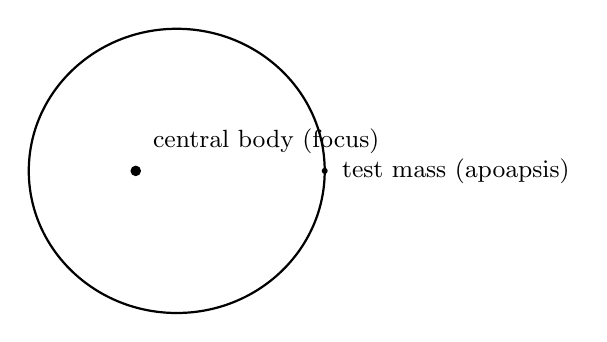
\begin{tikzpicture}[scale=2.4]
    \draw[thick] (0.217,0) ellipse [x radius=0.783, y radius=0.752];
    \fill (0,0) circle (0.028);
    \node[anchor=south west] at (0.04,0.04) {\small central body (focus)};
    \fill (1.0,0) circle (0.016);
    \node[anchor=west] at (1.04,0) {\small test mass (apoapsis)};
  \end{tikzpicture}
  \caption{Bound orbit of the test mass (outer curve) about the fixed central
  body at the ellipse's focus (origin), drawn to scale in normalized units.
  Geometry from the launch in Table~\ref{tab:checks}: apoapsis at $r = 1$,
  semi-major axis $a = 0.783$, eccentricity $e = 0.278$. This is a schematic,
  not a data plot.}
  \label{fig:orbit}
\end{figure}

\section{Closing}

This example establishes no new fact about the world: it recovers Newton's
inverse-square law, Kepler's third law, and energy conservation of a bound
orbit, to the precision in Table~\ref{tab:checks}. Its function is to exercise
the template's workflow end to end -- formalism in Section~\ref{sec:formalism},
a symplectic integrator in Section~\ref{sec:integrator}, and checks with
pre-declared falsifiers in Section~\ref{sec:verification} -- on a system whose
answers are already known.

\bibliographystyle{plainnat}
\bibliography{references}

\end{document}
